\usepackage[a4paper,top=25mm,bottom=25mm,left=28mm,right=24mm,headheight=22pt]{geometry}
\usepackage{fontspec}
\setmainfont{TeX Gyre Pagella}
\setsansfont{TeX Gyre Heros}
\setmonofont[Scale=MatchLowercase]{DejaVu Sans Mono}
\usepackage{microtype}
\usepackage{xcolor}
\definecolor{REMBlue}{HTML}{174A63}
\definecolor{REMRed}{HTML}{A33A2B}
\definecolor{REMCode}{HTML}{F4F6F7}
\usepackage{tikz}
\usetikzlibrary{arrows.meta,positioning}
\newcommand{\REMSoftwareStack}{%
  \begin{center}
  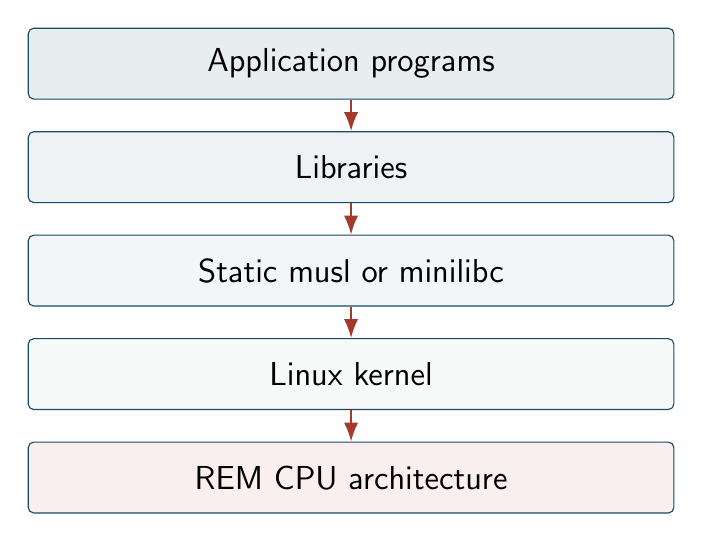
\begin{tikzpicture}[
    rembox/.style={draw=REMBlue, rounded corners=2pt, minimum width=82mm,
      minimum height=9mm, align=center, font=\sffamily\large},
    remarrow/.style={-{Latex[length=2.4mm]}, line width=0.7pt, draw=REMRed}]
    \node[rembox, fill=REMBlue!10] (app) {Application programs};
    \node[rembox, fill=REMBlue!7, below=4mm of app] (lib) {Libraries};
    \node[rembox, fill=REMBlue!5, below=4mm of lib] (libc) {Static musl or minilibc};
    \node[rembox, fill=REMBlue!3, below=4mm of libc] (kernel) {Linux kernel};
    \node[rembox, fill=REMRed!8, below=4mm of kernel] (cpu) {REM CPU architecture};
    \draw[remarrow] (app) -- (lib);
    \draw[remarrow] (lib) -- (libc);
    \draw[remarrow] (libc) -- (kernel);
    \draw[remarrow] (kernel) -- (cpu);
  \end{tikzpicture}
  \end{center}%
}
\newcommand{\REMFlowFive}[5]{%
  \begin{center}
  \begin{tikzpicture}[
    remflowbox/.style={draw=REMBlue, rounded corners=2pt, minimum width=55mm,
      minimum height=8mm, align=center, font=\sffamily\normalsize},
    remflowarrow/.style={-{Latex[length=2.2mm]}, line width=0.65pt, draw=REMRed}]
    \node[remflowbox, fill=REMBlue!7] (f1) {#1};
    \node[remflowbox, fill=REMBlue!7, below=3mm of f1] (f2) {#2};
    \node[remflowbox, fill=REMBlue!7, below=3mm of f2] (f3) {#3};
    \node[remflowbox, fill=REMBlue!7, below=3mm of f3] (f4) {#4};
    \node[remflowbox, fill=REMRed!8, below=3mm of f4] (f5) {#5};
    \draw[remflowarrow] (f1) -- (f2);
    \draw[remflowarrow] (f2) -- (f3);
    \draw[remflowarrow] (f3) -- (f4);
    \draw[remflowarrow] (f4) -- (f5);
  \end{tikzpicture}
  \end{center}%
}
\newcommand{\REMFlowThree}[3]{%
  \begin{center}
  \begin{tikzpicture}[
    remflowbox/.style={draw=REMBlue, rounded corners=2pt, minimum width=55mm,
      minimum height=8mm, align=center, font=\sffamily\normalsize},
    remflowarrow/.style={-{Latex[length=2.2mm]}, line width=0.65pt, draw=REMRed}]
    \node[remflowbox, fill=REMBlue!7] (f1) {#1};
    \node[remflowbox, fill=REMBlue!7, below=3mm of f1] (f2) {#2};
    \node[remflowbox, fill=REMRed!8, below=3mm of f2] (f3) {#3};
    \draw[remflowarrow] (f1) -- (f2);
    \draw[remflowarrow] (f2) -- (f3);
  \end{tikzpicture}
  \end{center}%
}
\newcommand{\REMFlowFour}[4]{%
  \begin{center}
  \begin{tikzpicture}[
    remflowbox/.style={draw=REMBlue, rounded corners=2pt, minimum width=55mm,
      minimum height=8mm, align=center, font=\sffamily\normalsize},
    remflowarrow/.style={-{Latex[length=2.2mm]}, line width=0.65pt, draw=REMRed}]
    \node[remflowbox, fill=REMBlue!7] (f1) {#1};
    \node[remflowbox, fill=REMBlue!7, below=3mm of f1] (f2) {#2};
    \node[remflowbox, fill=REMBlue!7, below=3mm of f2] (f3) {#3};
    \node[remflowbox, fill=REMRed!8, below=3mm of f3] (f4) {#4};
    \draw[remflowarrow] (f1) -- (f2);
    \draw[remflowarrow] (f2) -- (f3);
    \draw[remflowarrow] (f3) -- (f4);
  \end{tikzpicture}
  \end{center}%
}
\newcommand{\REMHorizontalFive}[5]{%
  \begin{center}
  \begin{tikzpicture}[
    remhbox/.style={draw=REMBlue, rounded corners=2pt, minimum width=27mm,
      minimum height=11mm, align=center, font=\sffamily\small},
    remharrow/.style={-{Latex[length=2.1mm]}, line width=0.65pt, draw=REMRed}]
    \node[remhbox, fill=REMBlue!7] (h1) {#1};
    \node[remhbox, fill=REMBlue!7, right=4mm of h1] (h2) {#2};
    \node[remhbox, fill=REMBlue!7, right=4mm of h2] (h3) {#3};
    \node[remhbox, fill=REMBlue!7, right=4mm of h3] (h4) {#4};
    \node[remhbox, fill=REMRed!8, right=4mm of h4] (h5) {#5};
    \draw[remharrow] (h1) -- (h2);
    \draw[remharrow] (h2) -- (h3);
    \draw[remharrow] (h3) -- (h4);
    \draw[remharrow] (h4) -- (h5);
  \end{tikzpicture}
  \end{center}%
}
\newcommand{\REMHorizontalThree}[3]{%
  \begin{center}
  \begin{tikzpicture}[
    remhbox/.style={draw=REMBlue, rounded corners=2pt, minimum width=39mm,
      minimum height=11mm, align=center, font=\sffamily\small},
    remharrow/.style={-{Latex[length=2.1mm]}, line width=0.65pt, draw=REMRed}]
    \node[remhbox, fill=REMBlue!7] (h1) {#1};
    \node[remhbox, fill=REMBlue!7, right=5mm of h1] (h2) {#2};
    \node[remhbox, fill=REMRed!8, right=5mm of h2] (h3) {#3};
    \draw[remharrow] (h1) -- (h2);
    \draw[remharrow] (h2) -- (h3);
  \end{tikzpicture}
  \end{center}%
}
\newcommand{\REMBytesThree}[3]{%
  \begin{center}
  \begin{tikzpicture}[
    rembyte/.style={draw=REMBlue, rounded corners=2pt, minimum width=18mm,
      minimum height=9mm, align=center, font=\ttfamily\small},
    rembytearrow/.style={-{Latex[length=2mm]}, line width=0.6pt, draw=REMRed}]
    \node[rembyte, fill=REMRed!8] (b1) {#1};
    \node[rembyte, fill=REMBlue!7, right=3mm of b1] (b2) {#2};
    \node[rembyte, fill=REMBlue!7, right=3mm of b2] (b3) {#3};
    \draw[rembytearrow] (b1) -- (b2);
    \draw[rembytearrow] (b2) -- (b3);
  \end{tikzpicture}
  \end{center}%
}
\newcommand{\REMBytesSix}[6]{%
  \begin{center}
  \begin{tikzpicture}[
    rembyte/.style={draw=REMBlue, rounded corners=2pt, minimum width=15mm,
      minimum height=9mm, align=center, font=\ttfamily\small},
    rembytearrow/.style={-{Latex[length=1.8mm]}, line width=0.55pt, draw=REMRed}]
    \node[rembyte, fill=REMRed!8] (b1) {#1};
    \node[rembyte, fill=REMBlue!7, right=2mm of b1] (b2) {#2};
    \node[rembyte, fill=REMBlue!7, right=2mm of b2] (b3) {#3};
    \node[rembyte, fill=REMBlue!7, right=2mm of b3] (b4) {#4};
    \node[rembyte, fill=REMBlue!7, right=2mm of b4] (b5) {#5};
    \node[rembyte, fill=REMBlue!7, right=2mm of b5] (b6) {#6};
    \draw[rembytearrow] (b1) -- (b2);
    \draw[rembytearrow] (b2) -- (b3);
    \draw[rembytearrow] (b3) -- (b4);
    \draw[rembytearrow] (b4) -- (b5);
    \draw[rembytearrow] (b5) -- (b6);
  \end{tikzpicture}
  \end{center}%
}
\newcommand{\REMBytesFour}[4]{%
  \begin{center}
  \begin{tikzpicture}[
    rembyte/.style={draw=REMBlue, rounded corners=2pt, minimum width=18mm,
      minimum height=9mm, align=center, font=\ttfamily\small},
    rembytearrow/.style={-{Latex[length=2mm]}, line width=0.6pt, draw=REMRed}]
    \node[rembyte, fill=REMRed!8] (b1) {#1};
    \node[rembyte, fill=REMBlue!7, right=3mm of b1] (b2) {#2};
    \node[rembyte, fill=REMBlue!7, right=3mm of b2] (b3) {#3};
    \node[rembyte, fill=REMBlue!7, right=3mm of b3] (b4) {#4};
    \draw[rembytearrow] (b1) -- (b2);
    \draw[rembytearrow] (b2) -- (b3);
    \draw[rembytearrow] (b3) -- (b4);
  \end{tikzpicture}
  \end{center}%
}
\usepackage{titlesec}
\titleformat{\chapter}[display]
  {\normalfont\sffamily\bfseries\color{REMBlue}}
  {\fontsize{13}{16}\selectfont\chaptertitlename\ \thechapter}
  {8pt}{\raggedright\fontsize{28}{32}\selectfont}
\titlespacing*{\chapter}{0pt}{-20pt}{24pt}
\titleformat{\section}
  {\normalfont\sffamily\Large\bfseries\color{REMBlue}}
  {\thesection}{0.7em}{}
\titleformat{\subsection}
  {\normalfont\sffamily\large\bfseries\color{REMRed}}
  {\thesubsection}{0.7em}{}
\usepackage{fancyhdr}
\pagestyle{fancy}
\fancyhf{}
\fancyhead[L]{\sffamily\small\nouppercase{\rightmark}}
\fancyhead[R]{\sffamily\small\thepage}
\renewcommand{\headrulewidth}{0.4pt}
\fancypagestyle{plain}{\fancyhf{}\fancyfoot[C]{\sffamily\small\thepage}\renewcommand{\headrulewidth}{0pt}}
\usepackage{booktabs}
\usepackage{longtable}
\usepackage{array}
\usepackage{etoolbox}
\AtBeginEnvironment{longtable}{\small}
\usepackage{enumitem}
\setlist{topsep=3pt,itemsep=2pt,parsep=0pt}
\usepackage{framed}
\definecolor{shadecolor}{HTML}{F4F6F7}
\usepackage{fvextra}
\RecustomVerbatimEnvironment{verbatim}{Verbatim}{breaklines=true,breakanywhere=true}
\usepackage{hyperref}
\hypersetup{colorlinks=true,linkcolor=REMBlue,urlcolor=REMRed,citecolor=REMBlue}
\usepackage{bookmark}
\setcounter{tocdepth}{0}
\renewcommand{\contentsname}{Contents}
\renewcommand{\partname}{Part}
\setlength{\emergencystretch}{3em}
\sloppy
